\documentclass[a4paper, 11pt, ngerman, fleqn]{article}
\usepackage[utf8]{inputenc}
\usepackage[ngerman]{babel}
\usepackage{ngerman}
\usepackage{coordsys,logsys,color}
\usepackage{german,fancyhdr}
\usepackage{hyperref}
\usepackage{texdraw}
\usepackage{graphicx}
\usepackage{caption}
\usepackage{subcaption}
\usepackage[printonlyused,withpage]{acronym}

\NeedsTeXFormat{LaTeX2e}
\ProvidesPackage{hyperref}
\definecolor{darkblue}{rgb}{0,0,.6}
\hypersetup{pdftex=false, colorlinks=true, breaklinks=true, linkcolor=darkblue, menucolor=darkblue, pagecolor=darkblue, urlcolor=darkblue, citecolor=darkblue}

\pagestyle{fancy}

\renewcommand{\familydefault}{cmss}

\definecolor{fgcgray}{rgb}{0.4, 0.4, 0.4}
\definecolor{warning}{rgb}{0.9, 0.1, 0.0}
\definecolor{bgctitle}{rgb}{0.5, 0.5, 0.5}
\definecolor{fgctitle}{rgb}{0.95, 0.95, 0.95}
\newcommand{\titlefont}[1]{\textcolor{fgctitle}{\fontfamily{cmss}\fontseries{bx}\fontshape{n}\fontsize{20.48}{0pt} \selectfont #1}}
\newcommand{\inversetitlefont}[1]{\textcolor{bgctitle}{\fontfamily{cmss}\fontseries{bx}\fontshape{n}\fontsize{20.48}{0pt} \selectfont #1}}

\addtolength{\oddsidemargin}{-1.0cm}
\addtolength{\evensidemargin}{-1.0cm}
\addtolength{\headwidth}{2.0cm}
\addtolength{\textwidth}{2.0cm}

\setlength{\parindent}{0cm}

\renewcommand{\labelitemi}{$\circ$}
\renewcommand{\labelitemii}{$\diamond$}

\newcommand{\spaceline}[1][8pt]{\vskip #1}
\newcommand{\comment}[1]{\spaceline[5pt] \textcolor{fgcgray}{\scriptsize #1} \spaceline[15pt]}
\newcommand{\attrname}[1]{\textcolor{fgcgray}{\scriptsize #1}}


\makeatletter

\newcommand*{\project}[1]{\gdef\@project{#1}}
\newcommand*{\version}[1]{\gdef\@version{#1}}
\newcommand*{\home}[1]{\gdef\@home{#1}}
\newcommand*{\homeref}[1]{\gdef\@homeref{#1}}
\newcommand*{\prerequisite}[1]{\gdef\@prerequisite{#1}}
\newcommand*{\prerequisiteref}[1]{\gdef\@prerequisiteref{#1}}

\def\@maketitle{
  %\begin{titlepage}
  \begin{center}
    \colorbox{bgctitle}{
      \parbox{\textwidth}{
        \spaceline
        \centering{\titlefont{\@title}}
        \par
        \spaceline
      }
    }
    \colorbox{white}{
      \parbox{\textwidth}{
        \spaceline
        \centering{\inversetitlefont{\@project}}
        \par
        \spaceline
      }
    }
  \end{center}
  \spaceline[1.5em] { 
    \begin{flushright}
    \begin{tabular}[t]{rl}
      \attrname{Projekt:} & \@project \\
      \attrname{Voraussetzung:}& \@prerequisite \\
      \attrname{Autoren:} & \@author \\
      \attrname{} & {\@home} \\
      \attrname{letzte "Anderung:} & \@date
    \end{tabular}
    \end{flushright}
    \par
  }
  \spaceline[5.5em]
  %\end{titlepage}
}

\setcounter{secnumdepth}{4}
\setcounter{tocdepth}{4}
	 
\newcounter{subsubsubsection}[subsubsection]
\def\subsubsubsectionmark#1{}
\def\thesubsubsubsection{\thesubsubsection .\arabic{subsubsubsection}}
\def\subsubsubsection{\@startsection{subsubsubsection}{4}{\z@}{-3.25ex plus -1 ex minus -.2ex}{1.5ex plus .2ex}{\normalsize\bf}}
\def\l@subsubsubsection{\@dottedtocline{4}{4.8em}{4.2em}}

\makeatother

\everytexdraw{
  \drawdim cm \linewd 0.01
  \arrowheadtype t:T
  \arrowheadsize l:0.2 w:0.2
  \setgray 0.5
}

\newcommand{\xheight}{0.6}
\newcommand{\xlength}{0.6}
\newcommand{\yheighta}{1.0}
\newcommand{\yheightb}{0.8}
\newcommand{\yheightc}{0.6}
\newcommand{\yheightd}{0.5}
\newcommand{\yheighte}{0.4}
\newcommand{\yheightf}{0.35}

\newcommand{\xhline}{\rlvec({\xlength} 0)}
\newcommand{\xharrow}{\ravec(0.7 0)}
\newcommand{\xnext}{%\rlvec(0.05 0) \lpatt(0.04 0.04) \rlvec(0.15 0) \lpatt()
}

\newcommand{\xtext}[3][\xheight]{
  \bsegment
    \bsegment
      \setsegscale 0.5
      \textref h:L v:C  \htext({\xheight} -0.1){#3}
    \esegment
    \setsegscale 0.5 \lvec(0 #1)
    \setsegscale 1
    \rlvec(#2 0) \rlvec(0 -#1) \rlvec(-#2 0) \lvec(0 0)
    \savepos(#2 0)(*@x *@y)
  \esegment
  \move(*@x *@y)
}

\newcommand{\bxtext}[3][\xheight]{
  \setgray{0.1}
  \linewd{0.026}
  \xtext[\xheight]{#2}{#3}
  \linewd{0.01}
  \setgray{0.5}
}

\newcommand{\xstartpage}{\bxtext{2.1}{Startseite}}
\newcommand{\xmainpage}{\bxtext{2.3}{Hauptseite}}
\newcommand{\xusermenu}{\bxtext{2.9}{Benutzermenu}}
\newcommand{\xgamelist}{\bxtext{2.2}{Spieleliste}}
\newcommand{\xportfolio}{\bxtext{2.0}{Portfolio}}
\newcommand{\xaccount}{\xtext{3.8}{Kennung per \textsl{eMail}}}


\begin{document}
  \lhead{\sc{Entwurfsdokumentation SWP HydraClient}}
%\cfoot{-~\thepage~-}
\title{Entwurfsdokumentation}
\project{Smartphone-Client für das Anonymisierungssystem Hydra}
\version{1.0}
\prerequisite{Pflichtenheft}

\author{Carl-Christian von Dalnok, Felix Kettnaker, Jan Lemmen, Lukas Meinl,}
\home{Liam Pfannkuch, Philipp Schock, Jonathan Skopp, Alexander Wand}

\maketitle
 \newpage
  \tableofcontents \newpage
  \section{Einleitung}
Der \ac{HC} ist die Nutzerapplikation des \acp{HS}.
Er bietet dem Nutzer eine \ac{GUI}, mithilfe welcher er (nach Hydra-Spezifikationen) Nachrichten versenden bzw. empfangen kann.
\subsection{Entwurfsziele}

\begin{description}
	
	\item[Korrektheit:] 
	Messages werden durch den \ac{HC} vollständig und korrekt und an den gewünschten Adressaten übermittelt. Dabei ist die Implementierung des System frei von Fehlern, die die Anonymität oder Integrität der Nutzer gefährden könnten.
	
	\item [Sicherheit:] Nachrichten sind gemäß der Spezifikationen des \acp{HS} kryptographisch geschützt, sodass sie weder rückverfolgt, noch mitgelesen werden können.
	
	\item [Erweiterbarkeit:] Der \ac{HC} soll möglichst einfach um die zusätzlichen Wunschfunktionen erweiterbar sein.
	
	\item [Optimierbarkeit:] Im Zuge der Entwicklung soll Veränderungen von Komponenten des \ac{HC} zur Verbesserung des System leicht umzusetzen sein.
	Diese könnten sein: 
	\begin{itemize}
		\item Verbesserung der \ac{GUI}
		\item Verbesserung der Datenbank
		\item Verbesserung der kryptographischen Funktionen
		\item Allgemeine Bugfixes
	\end{itemize}
	\item [Lesbarkeit:] Laufende Kommentare im Code und eine ausführliche Dokumentation sollen dem besseren Verständnis des Systems dienen.
	
	\item [Effizienz:] Das System soll möglichst schonend für Akkuladung sowie Rechenkapazität sein.
	
	\item [Benutzerfreundlichkeit:]
	Die \ac{GUI} soll für Nutzer intuitiv bedienbar sein unter der Voraussetzung, dass sie bereits Erfahrung mit Messengerdiensten haben.

\end{description}\newpage
\subsection{Anforderungsanalyse}

Der \ac{HC} muss vollständig nach Hydra-Spezifikationen laufen.
Dabei müssen wir folgenden Anforderungen nachkommen: 
\begin{itemize}
	\item  \ac{gRPC} für Kommunikation mit \ac{DS} und dem Entry-Mix 
	\item \ac{ECDH} für Schlüsselaustausch über Setup-Pakete 
	\item \ac{AES} für die Authenticated Encryption der Setup-Pakete 
	\item Feistel-Netzwerk mit 12 Runden Threefish-1024 für \ac{OE}
	\item Größe der Setup-Pakete und \acp{CC}
\end{itemize}
\newpage
\subsection{Technologien und Entwicklungswerkzeuge}

\subsubsection{Programmiersprachen}
\textnormal{Für die \ac{GUI} und den \ac{MS} wird \textbf{Kotlin} verwendet, eine bevorzugte Programmiersprache für Android-Apps. Für Fragmentierung und Komprimierung, die \ac{E2EE}, \ac{OE} und \ac{gRPC} wird \textbf{C++} verwendet, welche eine bevorzugte Programmiersprache für die effiziente Implementierung von Anforderungen ist.}

\subsubsection{Plug-Ins}
\textnormal{Es wird \textbf{\ac{NDK}} verwendet, um Teile des Codes in C++ schreiben zu können und \textbf{CMake} zum erstellen von Makefiles. Außerdem wird als API \textbf{\ac{JNI}} verwendet, um eine Schnittstelle zwischen dem Code in Kotlin und C++ zu ermöglichen.}

\subsubsection{Bibliotheken}
\textnormal{Es wird \textbf{libcrypto++} verwendet, um auf cryptografische Algorithmen zugreifen zu können. Außerdem kommt \textbf{\ac{ECDH}} zum Einsatz, um Schlüssel zwischen den Kommunikationspartnern auszutauschen. Zudem wird  \textbf{\ac{gRPC}} verwendet, um sowohl mit dem Entrymix, als auch mit dem \ac{DS} zu kommunizieren.}

\subsubsection{Tools}
\textnormal{Für die Versionierung, Wiki und das Bugtracking verwenden wir \textbf{GitLab}, welches auf Basis von Git arbeitet.}
\newpage
\subsection{Machbarkeitsanalyse}

\begin{itemize}
	\item Benutzerkennung
		\begin{itemize}
			\item Hier handelt es sich um Wunschfunktionen. Die Passwort Abfrage lässt sich realisieren und ist so als machbar anzusehen.
		\end{itemize}
	
	\item Kontakte hinzufügen
		\begin{itemize}
			\item Die Funktion mit einem QR Code lässt sich mithilfe der Spring 5 API recht gut und solide implementieren. Daher ist auch diese Funktion als machbar anzusehen.
		\end{itemize}
	
	\item Kontaktverwaltung
		\begin{itemize}
			\item Die Verwaltung der Kontakte erfolgt über eine Datenbank. In dieser ist es möglich, Kontakte anzulegen und zu entfernen. Diese Funktion ist als machbar anzusehen.
		\end{itemize}
	
	\item Chatfunktionen
	 \begin{itemize}
		\item Alle Funktionen sind machbar. 
	\end{itemize}
	
	\item Personalisierung
	\begin{itemize}
		\item Hierbei handelt es sich um triviale Funktionen der GUI. Da Kotlin CSS unterstützt ist diese Funktion durchaus machbar.
	\end{itemize}
	
	\item Hydra Funktionen
	\begin{itemize}
		\item Alle Hydra Funktionen sind möglich und umsetzbar. 
	\end{itemize}
	
	\item Fragmentierungsfunktion
	\begin{itemize}
		\item Hierbei handelt es sich um eine Wunschfunktion. Diese wird auch als solche behandelt. Es ist machbar, Nachrichten zu komprimieren und in Segmente zu zerlegen.
	\end{itemize} 

	\item Kommunikationsfunktion
	\begin{itemize}
		\item Sämtliche Pflichtfunktionen unterliegen dem generellen Ziel der App und sind machbar.
	\end{itemize}



\end{itemize}

\newpage


 \newpage
  \section{Grobentwurf}
Im Folgenden wird beschrieben in welche Bestandteile der \ac{HC} zerlegt wurde, welche Aufgaben diese Bestandteile übernehmen und wie diese Bestandteile miteinander kommunizieren.
\subsection{Architekturmuster}
Die Systemzerlegung (siehe Abbildung \ref{fig:Bild1}) ist nach der \ac{MVC} Architektur aufgeteilt. Dabei entspricht die \ac{GUI} dem Viewer, der \ac{MS} dem Controller und die \ac{HCB} dem Model. Im Unterschied zu der klassischen \ac{MVC} Architektur ist hier die Logik des Systems im Model und nicht im Controller vertreten. 
\subsection{Systemzerlegung}
Der \ac{HC} wird in Komponenten zerlegt. 
Jede Komponente übernimmt dabei bestimmte Aufgaben. 
Die Komponenten kommunizieren dabei über definierte Schnittstellen.
Orangene Komponenten werden in Kotlin programmiert, graue Komponenten in C++.

\begin{figure}[h]
  \centering
     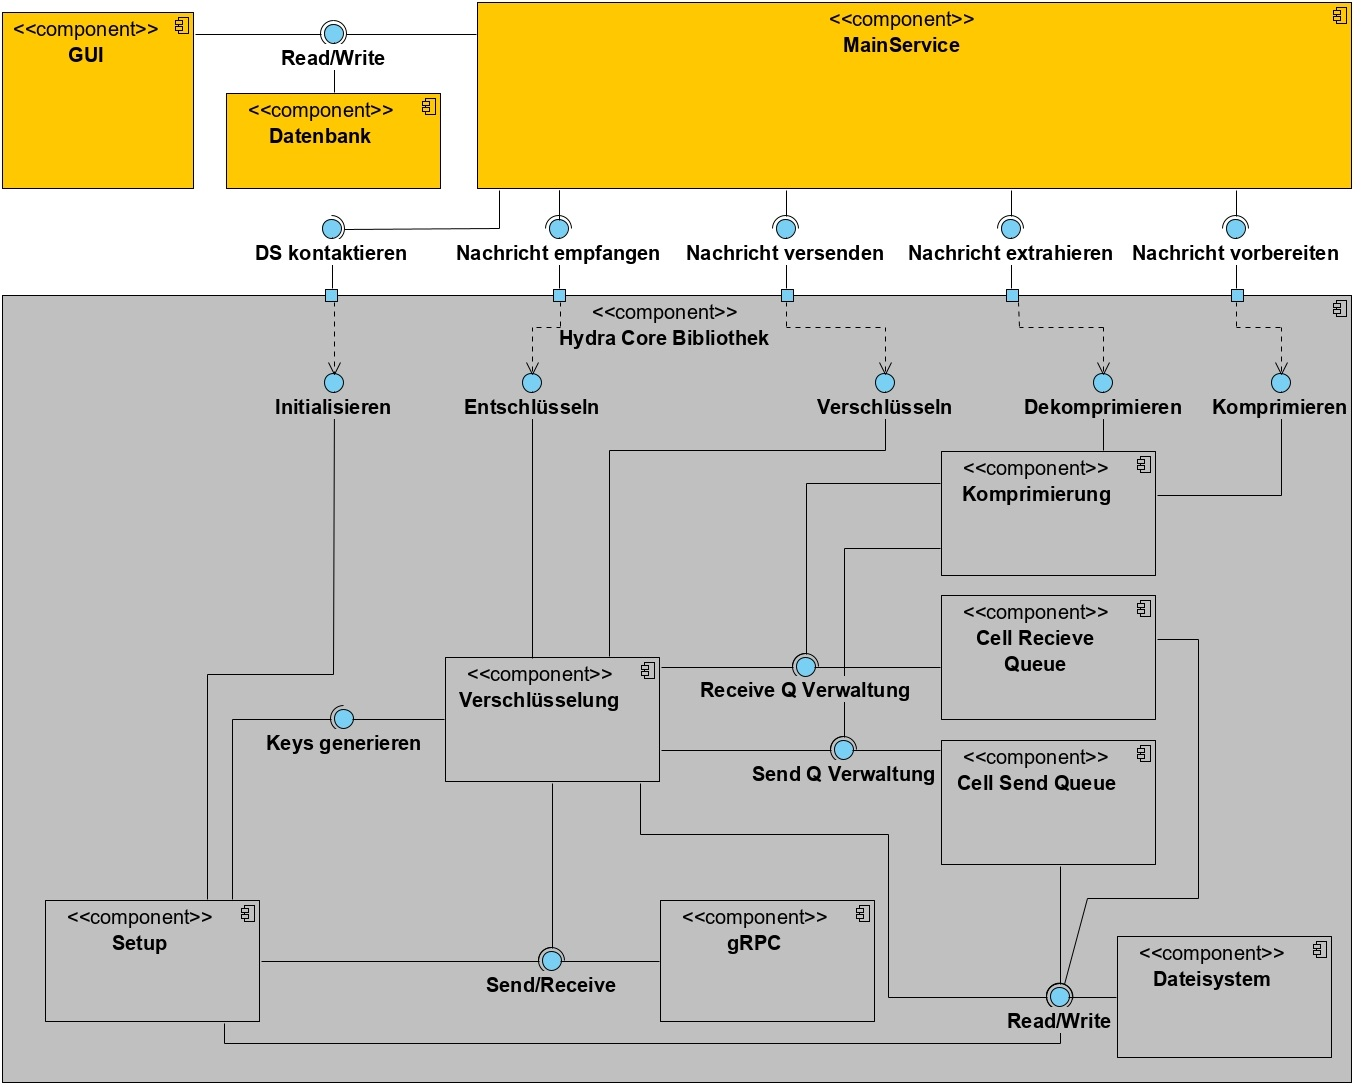
\includegraphics[width=0.9\textwidth]{diagramme/Component_Diagram_E2.jpg}
  \caption{Systemzerlegung des \acp{HC}}
  \label{fig:Bild1}
\end{figure}

\subsubsection{GUI-Activity}
Die \ac{GUI} stellt die Benutzerschnittelle dar, d.h. der Benutzer des \acp{HC} interagiert nur mit der \ac{GUI}. 
Die \ac{GUI} kommuniziert dabei nur mit der Datenbank, indem sie dort Einträge aktualisiert, hinzufügt oder löscht.
Für weitere Informationen siehe Abschnitt \ref{kap2_6:GUI}.

\subsubsection{Hydra Core Bibliothek}
Die \ac{HCB} beinhaltet alle wichtigen Funktionen, welche für das Hydra-Protokoll nötig sind. Sie generiert und verwaltet dabei ihre Daten selbst und kommuniziert mittels \ac{gRPC} mit dem \ac{HS}. Wichtig dabei ist, dass die \ac{HCB} passiv ist, d.h. sie nutzt keine Schnittstellen von anderen Komponenten.\\
\newline
Das Netzwerkinterface \ac{gRPC} bietet eine Schnittstelle für die Netzwerkoperationen senden bzw. empfangen einer Nachricht an. Des Weiteren wird über diese Schnittstelle mit dem \ac{DS} kommuniziert.\\
\newline
Das Dateisystem bietet eine Schnittelle für Lese- und Schreibzugriffe auf persistente Daten an.\\
\newline
Das Setup verbindet sich über \ac{gRPC} mit dem \ac{DS}, ruft die neuen Netzwerkinformationen (siehe Pflichtenheft Kapitel 4.2 /F0510/) von diesem ab und aktualisiert die im Dateisystem vorhandenen Daten. Des Weiteren erstellt das Setup die Setup-Pakete für zukünftige Epochen und versendet diese über \ac{gRPC} an die jeweiligen Mixe.\\
\newline
Bei dem Aufruf \textit{Nachricht vorbereiten} übergibt der \ac{MS} die vorzubereitende Nachricht an die Komprimierung. Diese komprimiert die übergebene Nachricht, indem sie die Textcodierung von UTF-16 in ASCII umwandelt, und gibt sie an die \ac{CSQ} weiter.
Bei dem Aufruf \textit{Nachricht extrahieren} entnimmt die Komponente eine Nachricht aus der \ac{CSQ}, dekomprimiert diese und gibt sie als Rückgabewert an den \ac{MS} zurück.\\
\newline
Die \ac{CSQ} nimmt eine komprimierte Nachricht der Komprimierung entgegen, reiht diese in die Warteschlange hinten ein und legt sie im Dateisystem ab. Auf Anfrage der Komponente Verschlüsselung nimmt die \ac{CSQ} die vorderste Nachricht der Warteschlange, übergibt diese der Verschlüsselung und löscht sie aus dem Dateisystem.\\
Die \ac{CSQ} übernimmt die Fragmentierung für Nachrichten, die für ein einzelnes Paket zu groß wären, reiht die einzelnen Fragmente korrekt in die Warteschlange ein und legt die Fragmente im Dateisystem ab. \\
Außerdem kümmert sie sich um die Zustellungsgarantie von Nachrichten. Sowohl die Zustellungsgarantie als auch die Fragmentierung werden nach TCP-Vorbild implementiert.\\
\newline

Die \ac{CRQ} nimmt ein Datenpaket der Verschlüsselung entgegen und legt dieses im Dateisystem ab. Handelt es sich bei dem Datenpaket um ein Fragment einer größeren Nachricht, so wird die \ac{CRQ} diese zu einer vollständigen Nachricht zusammensetzen, bevor die vollständige Nachricht an die Komprimierung weitergegeben werden kann.\\
\newline
Die Komponente Verschlüsselung generiert auf Anfrage die Schlüssel für das Setup.\\
Des Weiteren verschlüsselt sie Nachrichten mithilfe von \ac{AES} Ende-zu-Ende und generiert aus der verschlüsselten Nachricht eine \ac{CC}. Der Payload der \ac{CC} wird onion-encryptet mithilfe von einem Feistel-Netzwerk mit 12 Runden Threefish-1024.\\
Außerdem kann die Komponente sowohl die \ac{OE} als auch die \ac{E2EE} entfernen.
Die Komponente sendet bzw. empfängt \acp{CC} über \ac{gRPC}. Sie erkennt dabei auch manipulierte \acp{CC} bzw. \acp{DP} und verwirft diese. Ansonsten wird der Inhalt der \acp{CC} an die \ac{CRQ} übermittelt.
Bei dem Aufruf \textit{Nachricht empfangen} gibt die Komponente zurück, ob es eine vollständige Nachricht, ein Fragment oder eine ungültige Nachricht empfangen hat.

\subsubsection{Main-Service}
Der \ac{MS} ist für die Steuerung der Programmabläufe verantwortlich. Somit hat er insgesamt drei Schnittstellen:
\begin{itemize}
\item[1)]Der \ac{MS} kommuniziert mit der Datenbank und kann so indirekt Informationen mit der \ac{GUI} austauschen.
\item[2)]Der \ac{MS} kommuniziert mithilfe des \acp{NDK} mit der \ac{HCB} über einfache, synchrone Methodenaufrufe.
\end{itemize}
Als einzige Komponente kann der \ac{MS} sowohl mit der \ac{GUI} als auch mit der \ac{HCB} kommunizieren.\newpage
\subsection{Entwurfsalternativen}
Neben dem in Abbildung \ref{fig:Bild1} gezeigten Entwurf gibt es drei andere Alternativen. Die ersten beiden Entwurfsalternativen beziehen sich dabei nur auf die Aufteilung, welche Komponenten in welcher Programmiersprache programmiert werden. Die dritte Alternative bezieht sich dabei auf die Datenbank.
\subsubsection{1. Entwurfsalternative}

\begin{figure}[h]
  \centering
     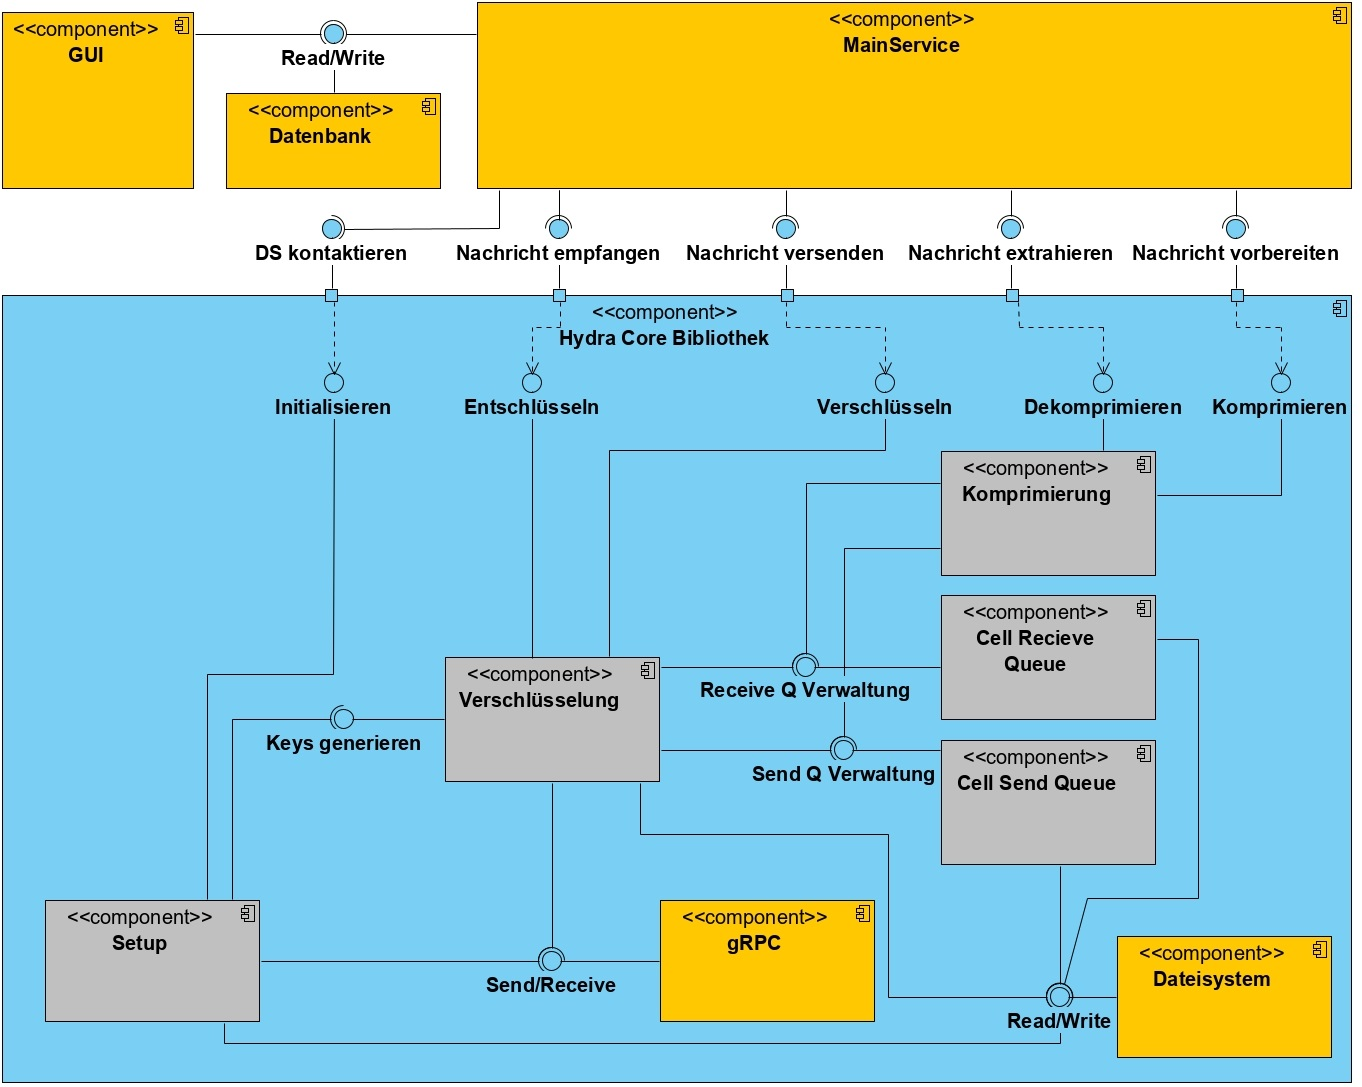
\includegraphics[width=0.9\textwidth]{diagramme/Component_Diagram_E1.jpg}
  \caption{1. Entwurfsalternative}
  \label{fig:Bild2}
\end{figure}

In der ersten Entwurfsalternative ist im Unterschied zu dem in Abbildung \ref{fig:Bild1} gezeigten Entwurf sowohl die Netzwerkschnittelle \ac{gRPC} als auch das Dateisystem  in Kotlin programmiert. Das Ganze hat aber entscheidende  Nachteile:
\begin{itemize}
\item[1)] Das Hydra-System schreibt uns \ac{gRPC} als Netzwerkschnittstelle vor und liefert uns bereits ein Protocol Buffer, welcher in C++ programmiert ist. Es wäre also unnötig, diese Komponente nochmals neu in Kotlin zu programmieren.
\item[2)]Das Dateisystem verwaltet in der \ac{HCB} ausschließlich Dateien, auf die Komponenten zugreifen, welche in C++ programmiert sind. Somit wäre es inkonsistent und unnötig kompliziert, das Dateisystem in Kotlin zu programmieren
\end{itemize}

Aus den genannten Gründen ist diese Entwurfsalternative ungeeignet.

\subsubsection{2. Entwurfsalternative}

\begin{figure}[h]
  \centering
     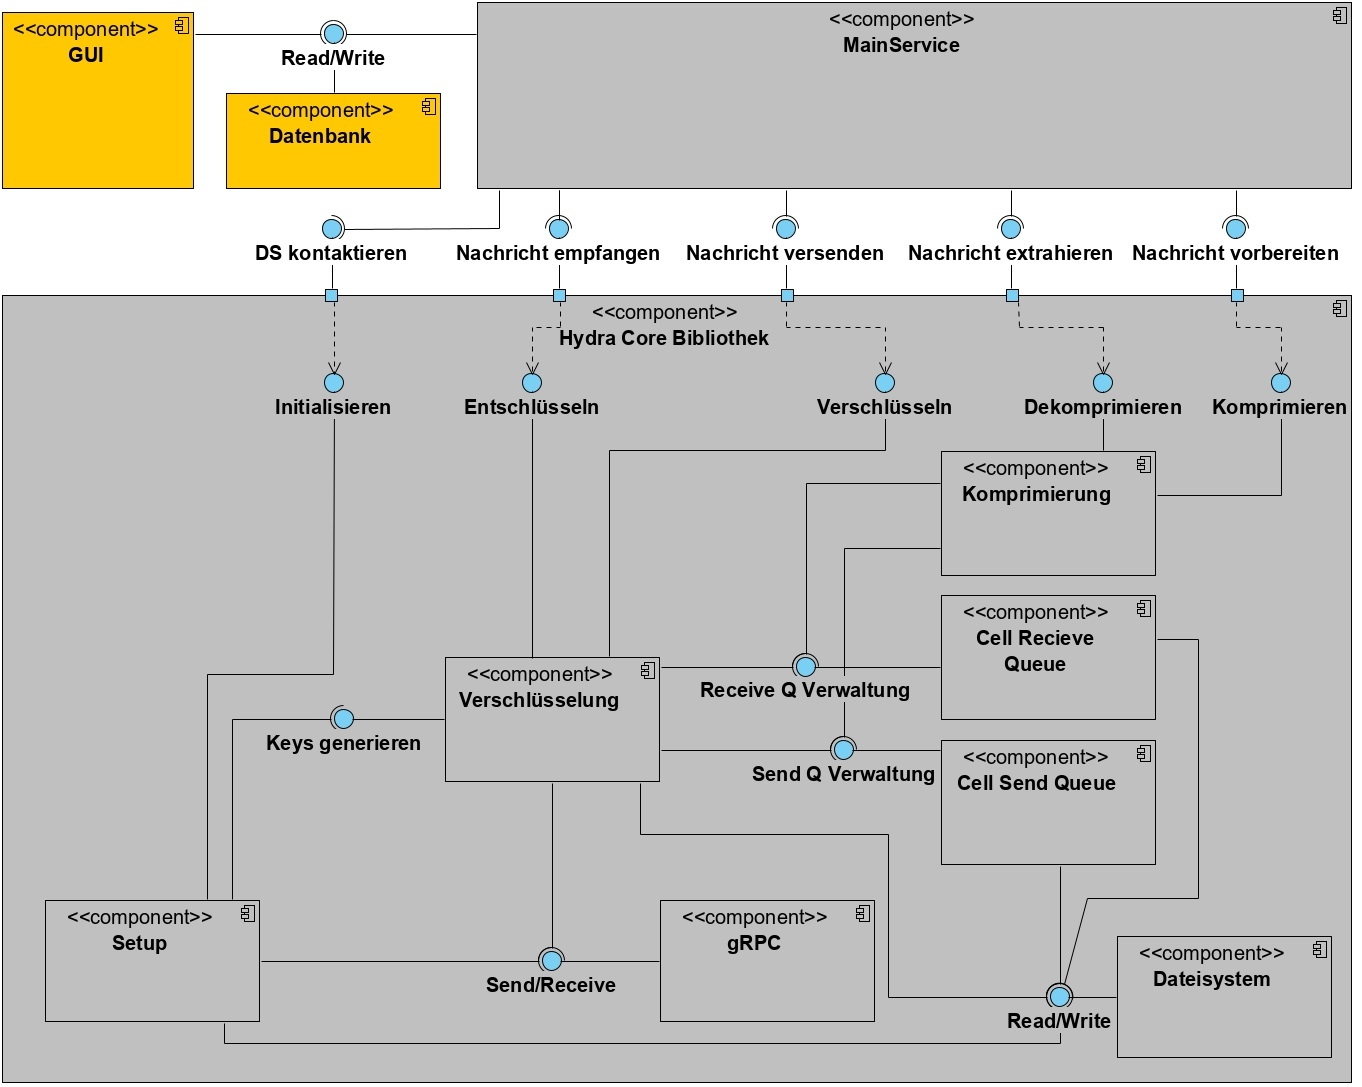
\includegraphics[width=0.9\textwidth]{diagramme/Component_Diagram_E3.jpg}
  \caption{2. Entwurfsalternative}
  \label{fig:Bild3}
\end{figure}

In der zweiten Entwurfsalternative ist neben der \ac{HCB} auch der \ac{MS} in C++ programmiert. Doch dies hat wieder einen entschiedenen Nachteil: Der \ac{MS} muss mit dem Android System kommunizieren. Da Kotlin extra für die Android-Entwicklung entwickelt worden ist, würde man das System nur unnötig schwer gestalten, wenn man den \ac{MS} in C++ programmiert. 

Aus diesem Grund ist auch diese Entwurfsalternative ungeeignet.
\newpage
\subsubsection{3. Entwurfsalternative}

\begin{figure}[h]
  \centering
     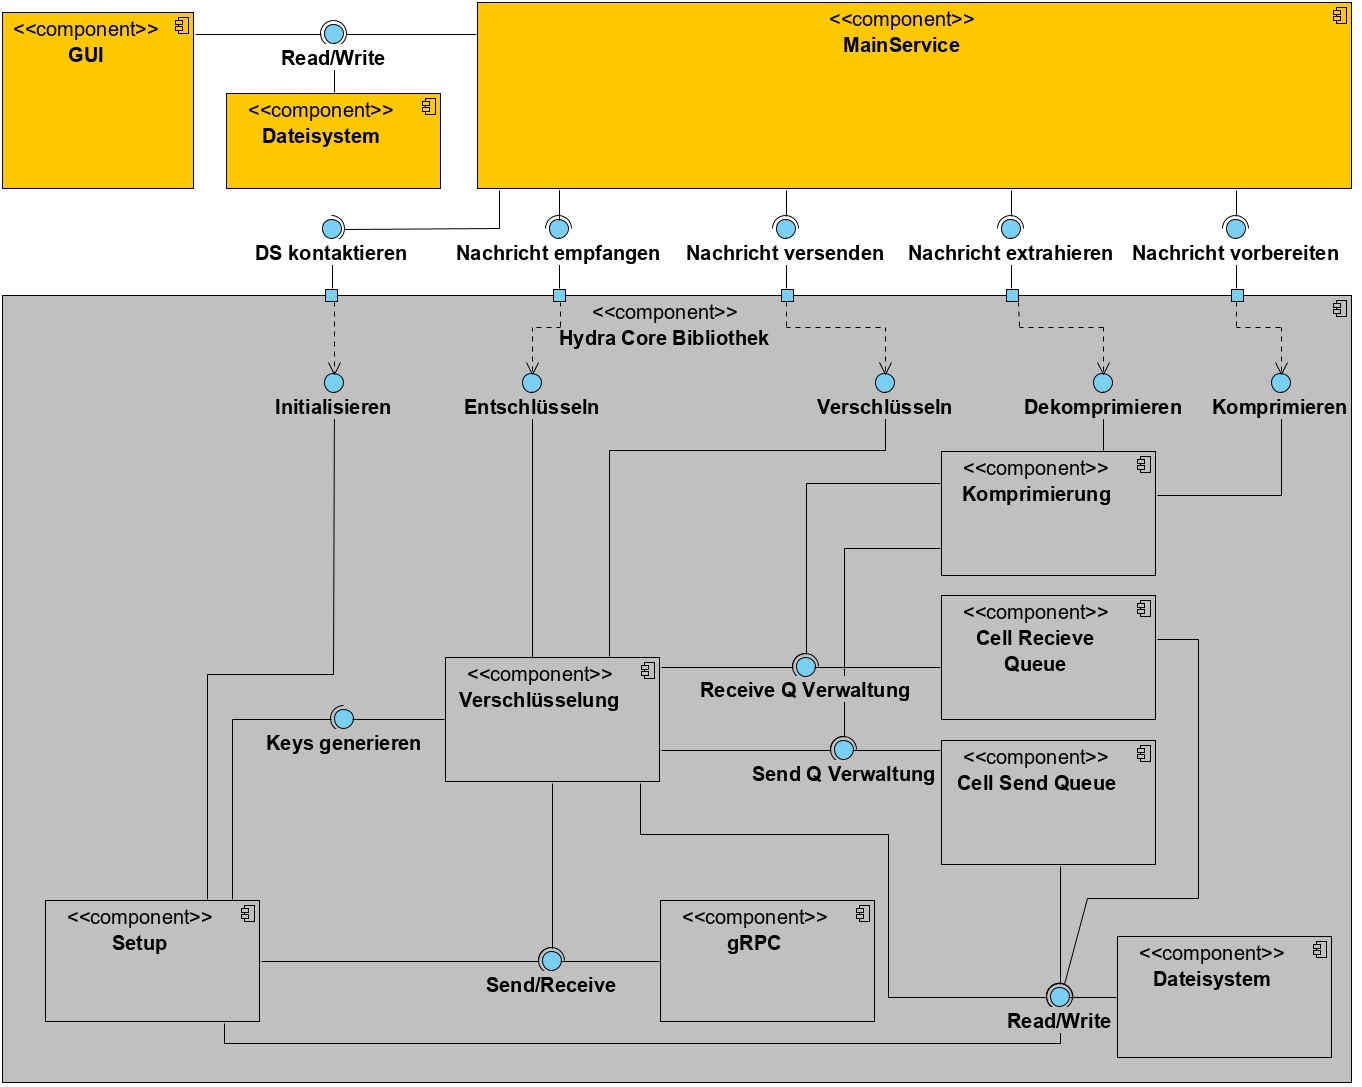
\includegraphics[width=0.9\textwidth]{diagramme/Component_Diagram_E4.jpg}
  \caption{3. Entwurfsalternative}
  \label{fig:Bild4}
\end{figure}

In der dritten Entwurfsalternative wird anstatt einer Datenbank ein einfaches Dateisystem genutzt. Aber auch diese Alternative hat mehrere Nachteile:
\begin{itemize}
\item[1)]Da sowohl der \ac{MS} also auch die \ac{GUI} auf den Chatverlauf bzw. das Kontaktbuch zugreifen, müsste ein wechselseitiger Ausschluss implementiert werden. 
\item[2)]Da die Kommunikation zwischen dem \ac{MS} und der \ac{GUI} über das Dateisystem läuft, müssen Such-Operationen ausgeführt werden (um neue Nachrichten zu entdecken usw.). Genau solche Operationen sind sehr effizient in Datenbanken implementiert und müssen hier selbst implementiert werden. 
\end{itemize}

Aus den genannten Gründen ist auch diese Entwurfsalternative eher ungeeignet.
\newpage
\subsection{Globaler Kontrollfluss}
Um den globalen Kontrollfluss des Systems zu verdeutlichen wird im Folgenden aufgezeigt, welche Schritte abgearbeitet werden, um Nachrichten zu empfangen, Nachrichten zu versenden und um den \ac{DS} zu kontaktieren . \\
 


\subsubsection{Nachricht versenden}

\begin{figure}[h]
  \centering
     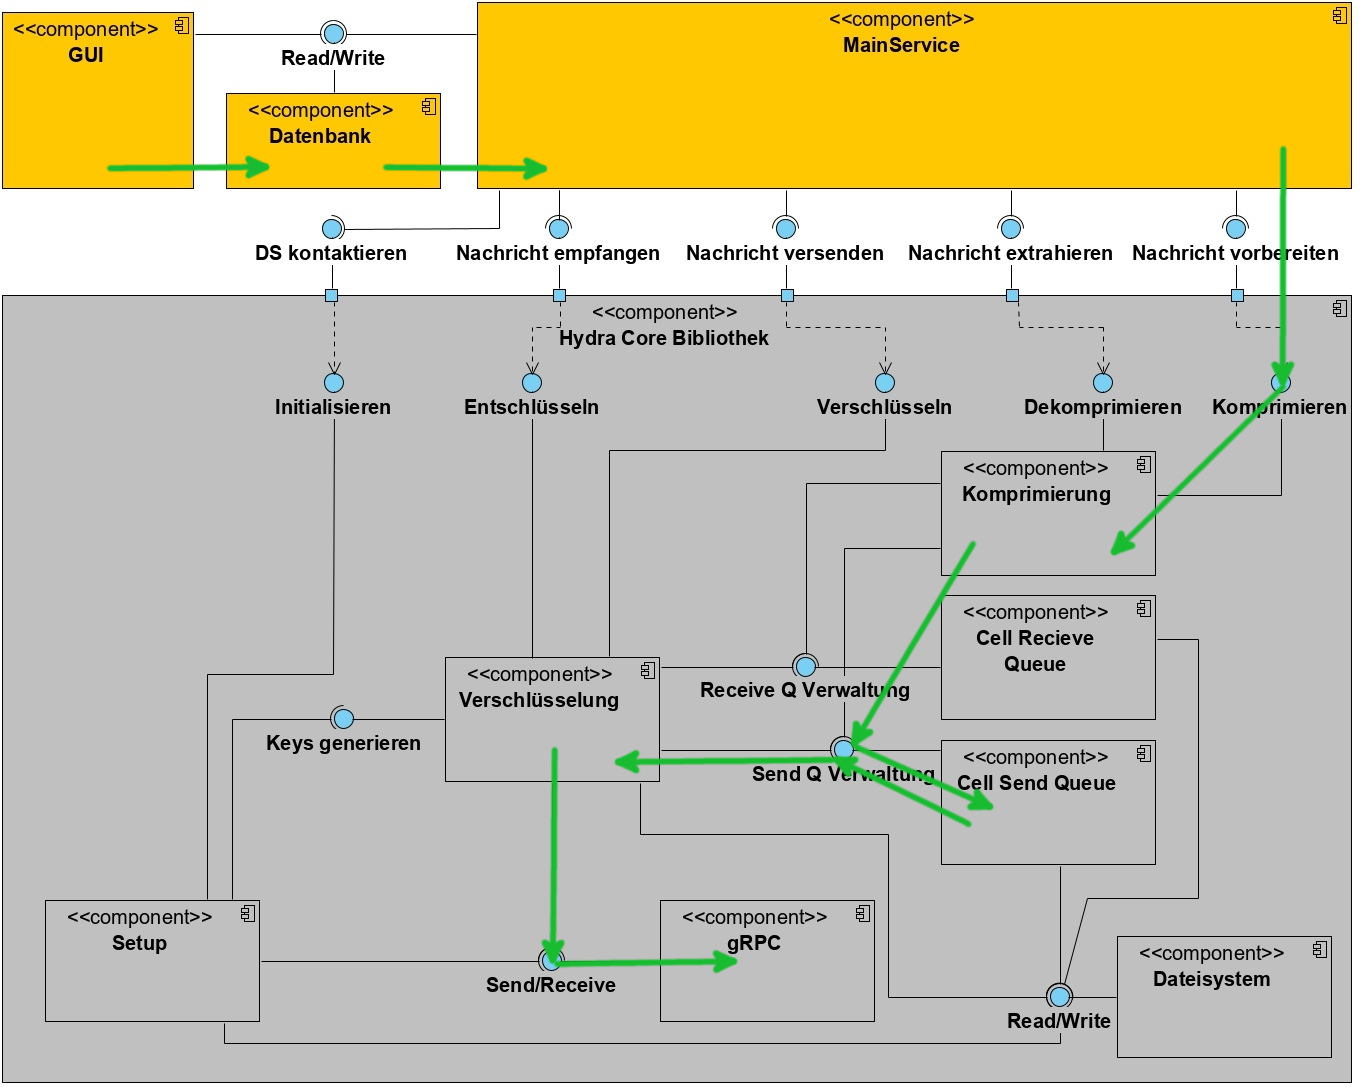
\includegraphics[width=0.9\textwidth]{diagramme/Glob_Kontrollfluss_1.jpg}
  \caption{Kontrollfluss Textnachricht versenden}
  \label{fig:Bild5}
\end{figure}

\begin{enumerate}
    \item
        Der Benutzer gibt eine Nachricht in die \ac{GUI} ein.

    \item
        Die Nachricht wird in der verschlüsselten Datenbank abgespeichert.

    \item
        Der \ac{MS} erkennt eine neue Nachricht in der Datenbank und übergibt sie der \ac{HCB}.

    \item
        Die Nachricht wird von UTF-16 zu ASCII komprimiert.

    \item
        Die Nachricht wird in der \ac{CSQ} abgelegt.

    \item
        Die Nachricht wird Fragment für Fragment aus der \ac{CSQ}  genommen. Anschließend wird eine \ac{E2EE} angewandt. Dazu verwenden wir \ac{AES}. Des Weiteren werden die Fragmente in Circuit-Cells gepackt und onion-encrypted.

    \item
        Die Cells werden anschließend mittels \ac{gRPC} versendet.
\end{enumerate}

\newpage
\subsubsection{Nachricht empfangen}

\begin{figure}[h]
  \centering
     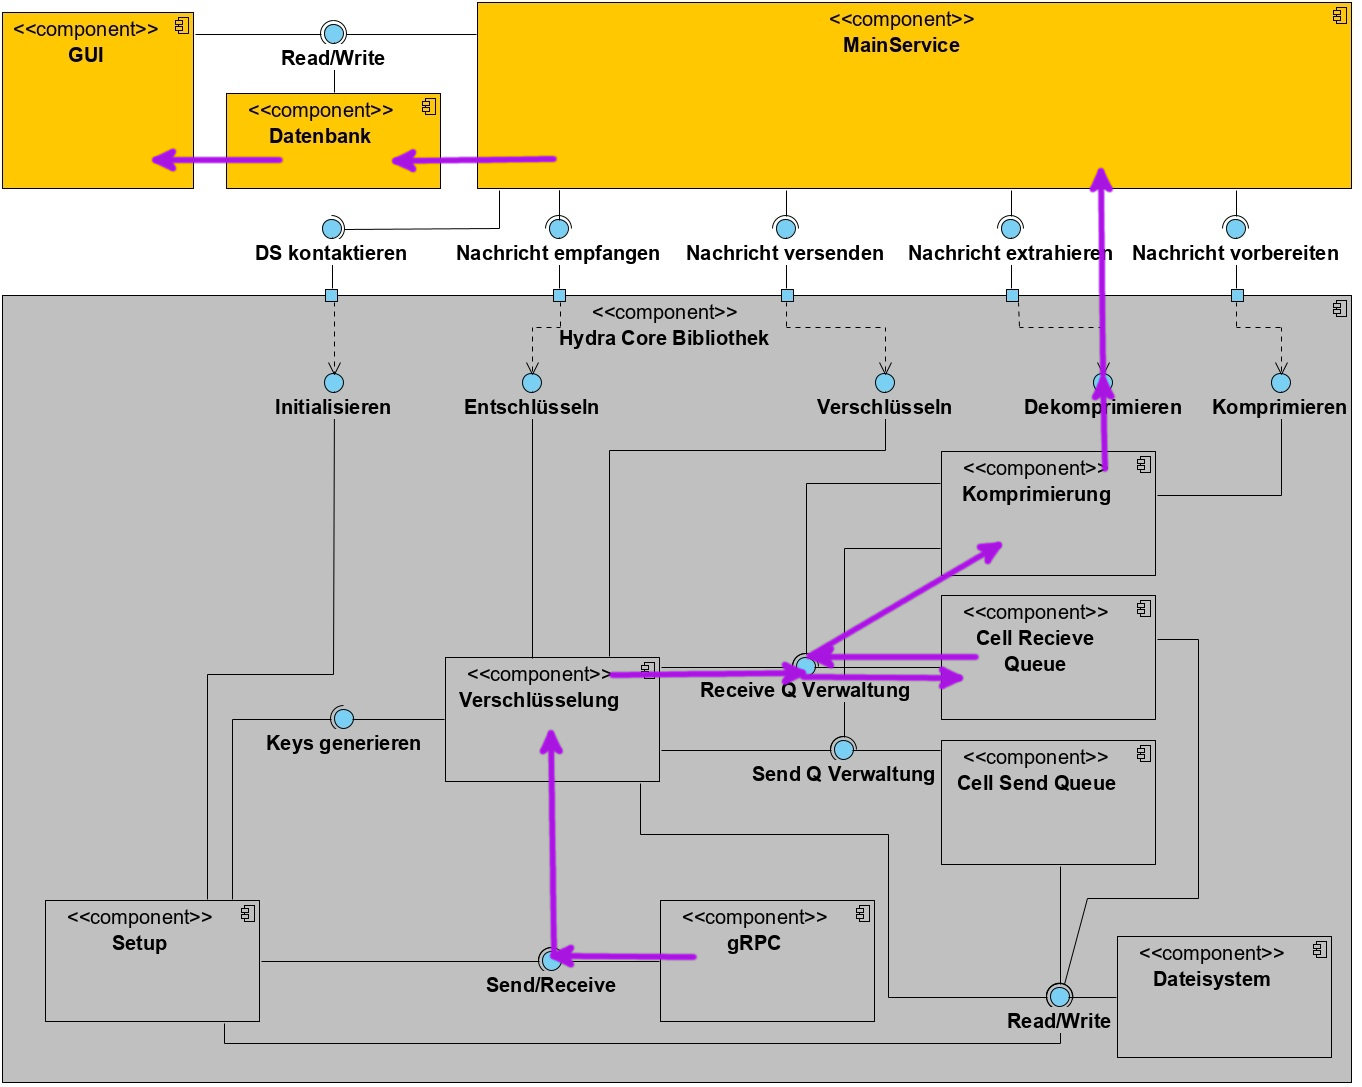
\includegraphics[width=0.9\textwidth]{diagramme/Glob_Kontrollfluss_2.jpg}
  \caption{Kontrollfluss Textnachricht empfangen}
  \label{fig:Bild6}
\end{figure}

\begin{enumerate}
    \item
        Die Cells werden mithilfe von \ac{gRPC} empfangen, dies gewährleistet die \ac{CSQ} des Senders.

    \item
        Die \ac{OE} und \ac{E2EE} werden entfernt.

    \item
        Die Nachricht wird Fragment für Fragment in die \ac{CRQ} geschrieben, bis alle Fragmente angekommen sind. Für jedes, in die \ac{CRQ} eingefügtes Fragment, wird ein Acknowledgement versendet.

    \item
        Die Nachricht wird dekomprimiert.

    \item
        Die Nachricht wird an den \ac{MS} übergeben.

    \item
        Der \ac{MS} speichert die Nachricht in der Datenbank.

    \item
        Die \ac{GUI} liest die Nachricht aus und zeigt sie dem Nutzer an.
\end{enumerate}

\newpage
\subsubsection{\ac{DS} kontaktieren}
 
 \begin{figure}[h]
  \centering
     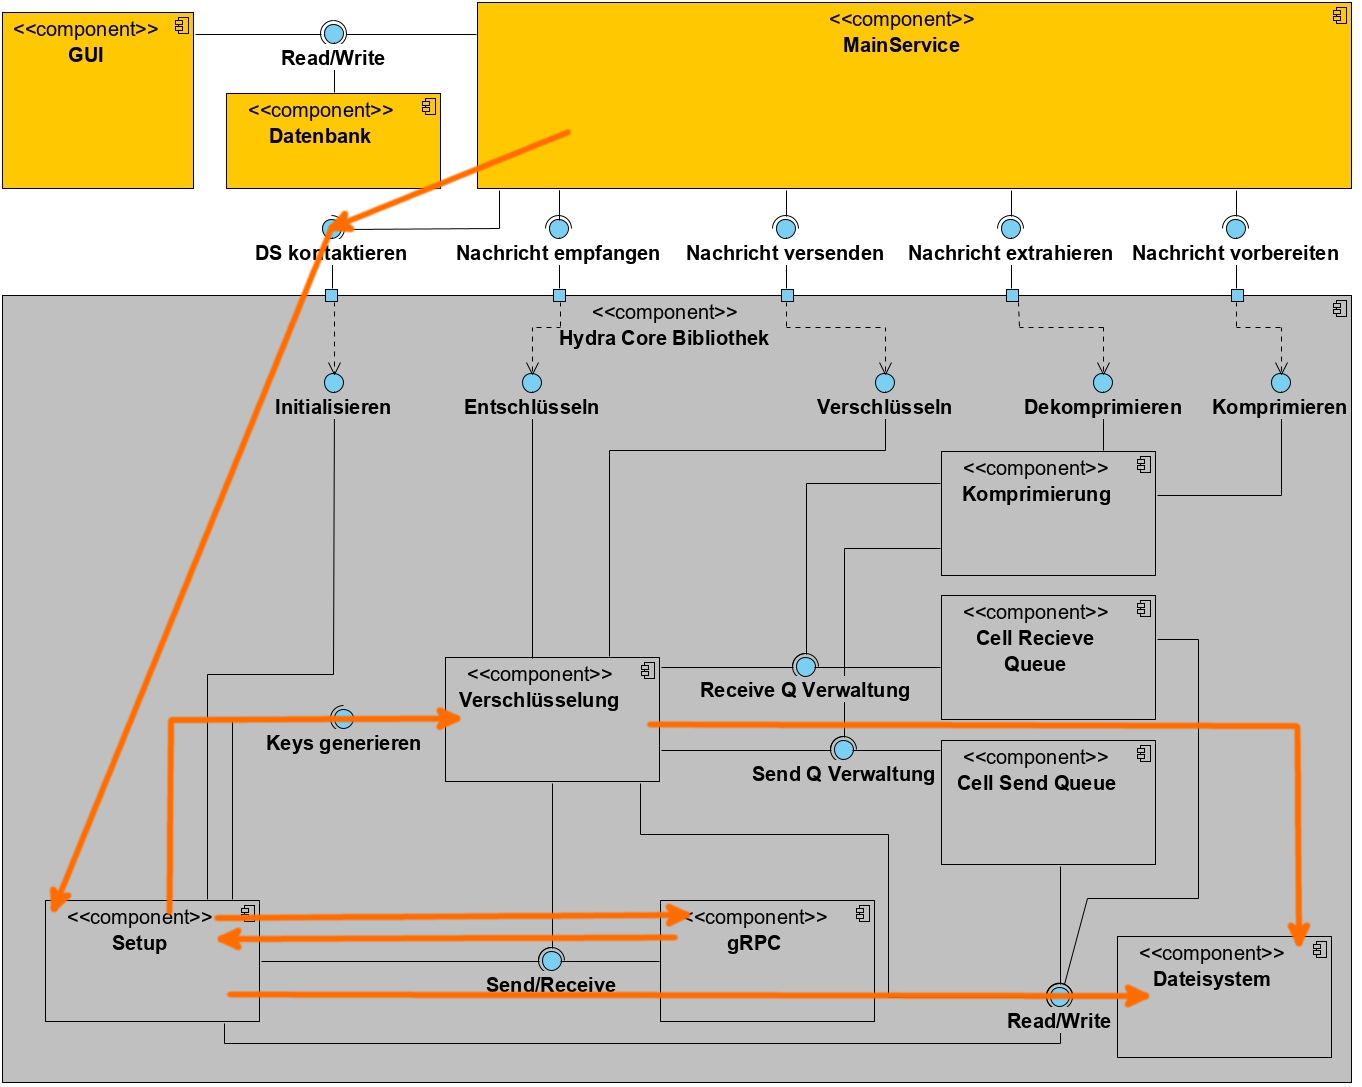
\includegraphics[width=0.9\textwidth]{diagramme/Glob_Kontrollfluss_3.jpg}
  \caption{Kontrollfluss \ac{DS} kontaktieren}
  \label{fig:Bild7}
\end{figure}

\begin{enumerate}
\item Der \ac{MS} ruft die Funktion \textit{\ac{DS} kontaktieren} auf.
\item Das Setup sendet eine Anfrage an der \ac{DS}.
\item Das Setup empfängt die Informationen vom \ac{DS}.
\item Das Setup aktualisiert die Informationen in der Directory-Datei.
\item Das Setup erzeugt für die neuen Epochen jeweils einen neuen Circuit. Dabei wird für jeden neuen Circuit ein Setup-Paket erstellt.
\item Das Setup sendet die erzeugten Setup-Pakets mithilfe von \ac{gRPC} an die dazugehörigen Entry-Mixe.
\item Das Setup lässt sich die neuen onion-Keys für die neuen Epochen von der Komponente \textit{Verschlüsselung} erzeugen und speichert diese in der CircuitKeys-Datei ab.
\end{enumerate}

\newpage
\subsection{Management persistenter Daten}

Die Speicherung der Daten erfolgt grundsätzlich in Form einer Datenbank für Kontakte mitsamt deren Chatverläufen und Nicknames. Des Weiteren gibt es \ac{CSQ} bzw. \ac{CRQ} und andere Dateien: Hash Chains der Kontakte, Directory (Info über Epochen) und Circuit Keys.
Das Kontaktbuch ist zweigeteilt, um Komplikationen zwischen den verschiedenen verwendeten Programmiersprachen bei gleichzeitigem Zugriff zu vermeiden. Deshalb gibt es eine KontaktID, welche zum Verbinden der Kontaktdaten dient.


\subsubsection{Verschlüsselung}
Die Verschlüsselung der persistenten Daten wird größtenteils vom Android Keystore System übernommen.
Dabei handelt es sich um einen von Android bereitgestellten Dienst, mit dessen Hilfe man kryptographische Schlüssel sicher abspeichern kann.
Zudem kann er auch benutzt werden, um Dateien verschlüsseln zu lassen.

Bei Dateien, welche vom Kotlin Teil verwaltet werden, wird die Verschlüsselung und das sichere Abspeichern der dafür benötigten Schlüssel komplett vom Keystore System übernommen.
Da die Verwendung des Keystore Systems bei C++ wesentlich schwieriger ist, als bei der Android nahestehenden Sprache Kotlin, wird hier anders verfahren.
Die Verschlüsselung der Dateien wird von eigenen Methoden der Core Bibliothek übernommen.
Der dafür notwendige Schlüssel wird vom Keystore System gespeichert und vom \ac{MS} bei C++ Methodenaufrufen als Parameter übergeben.

Sowohl das Keystore System, als auch die Core Bibliothek realisieren die Verschlüsselung durch AES.

\newpage
\subsubsection{Datenbank}
In der Datenbank ist das Kontaktbuch mit Kontakt IDs und dazugehörigen Nicknamen sowie Chatverläufen gespeichert.
Verschlüsselung erfolgt durch durch das Keystore System.
Zugriff erfolgt durch die \ac{GUI} und den \ac{MS}.

Das folgende ER-Modell beschreibt die Datenbank:

\begin{figure}[h]
  \centering
     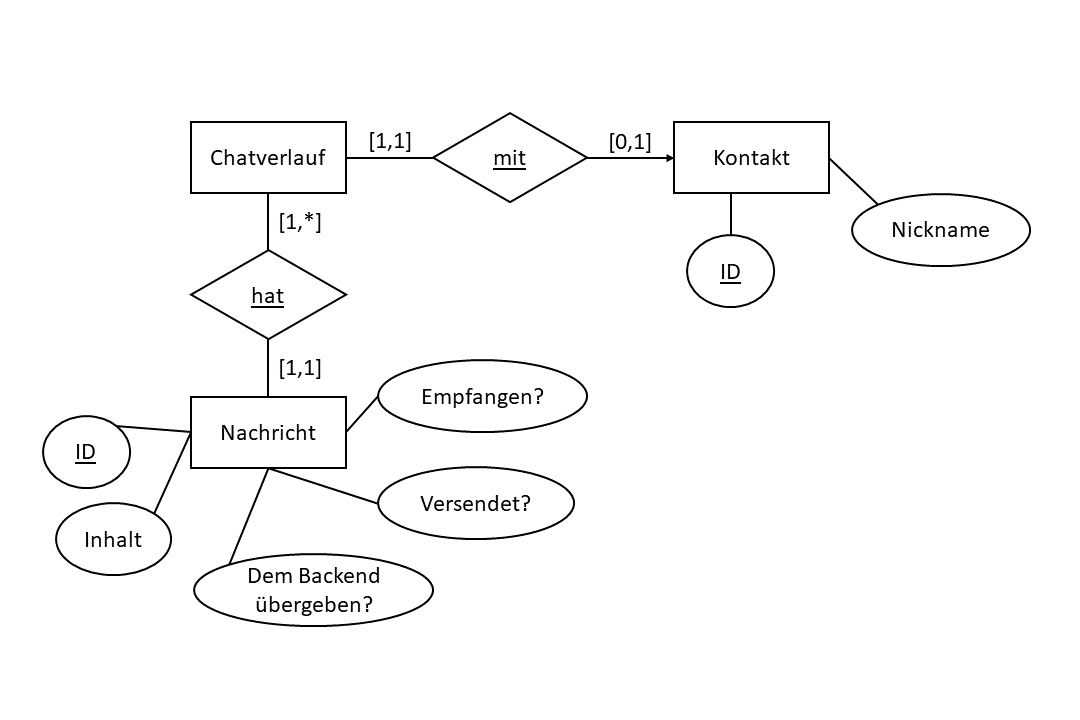
\includegraphics[width=0.9\textwidth]{diagramme/db.png}
  \caption{ER-Diagramm Datenbank}
  \label{fig:Bild8}
\end{figure}


\subsubsection{Kontakt Hash Chains}
\label{Kap2_3_2}
Im zweiten Teil des Kontaktbuchs sind Kontakt IDs mit zugehörigen gemeinsamen Schlüssel gespeichert.
Verschlüsselung erfolgt durch die Core Bibliothek.
Zugriff erfolgt durch das C++ Dateisystem.

\subsubsection{Directory}
Hier sind Informationen zu Epochen und Kommunikationsrunden gespeichert.
Da diese Daten öffentlich bekannt sind, ist diese Datei unverschlüsselt.
Zugriff erfolgt durch das C++ Dateisystem.

\subsubsection{Circuits}
In der Circuits Datei befinden sich die symmetrischen Schlüssel für die Mixe der gewählten Circuits für bestehende, sowie die kommenden Epochen.
Verschlüsselung erfolgt durch durch die Core Bibliothek.
Zugriff erfolgt durch das C++ Dateisystem.

\subsubsection{Cell Receive Queue}
\label{Kap2_3_6}
Dies ist eine Warteschlange, in der eingegangene, entschlüsselte Nachrichten, die noch entkomprimiert und ggf. defragmentiert werden müssen, zwischengespeichert werden.
Verschlüsselung erfolgt durch die Core Bibliothek.
Zugriff durch C++ Funktionen, die Verschlüsselung ausführen, sowie solche zur Fragmentierung und Komprimierung.

\subsubsection{Cell Send Queue}
Dies ist ein Warteschlange, in der komprimierte, ggf. fragmentierte Nachrichten, die versendet werden sollen, zwischengespeichert werden. 
Verschlüsselung erfolgt durch die Core Bibliothek.
Zugriff durch C++ Funktionen, die Verschlüsselung ausführen, sowie solche zur Fragmentierung und Komprimierung.
 \newpage
\subsection{GUI}
\label{kap2_6:GUI}
Im Folgenden werden ausschließlich die \ac{GUI}-Elemente dargestellt die für Pflichtfunktionen benötigt werden.\\


\begin{figure}[h]
\centering
\begin{subfigure}{.5\textwidth}
  \centering
  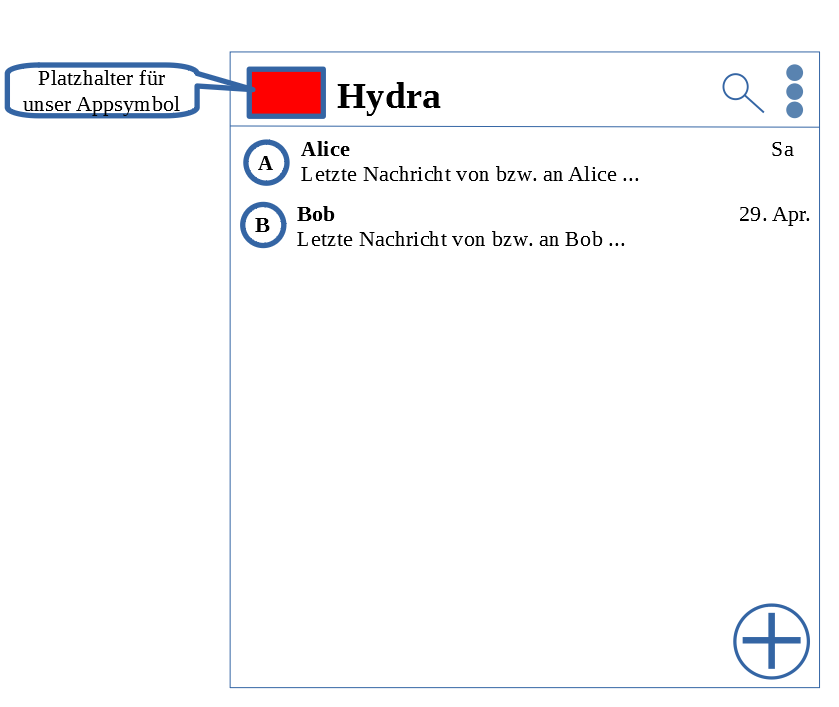
\includegraphics[scale=0.3]{gui/Startseite.png}
  \caption{Startseite}
\end{subfigure}%
\begin{subfigure}{.5\textwidth}
  \centering
  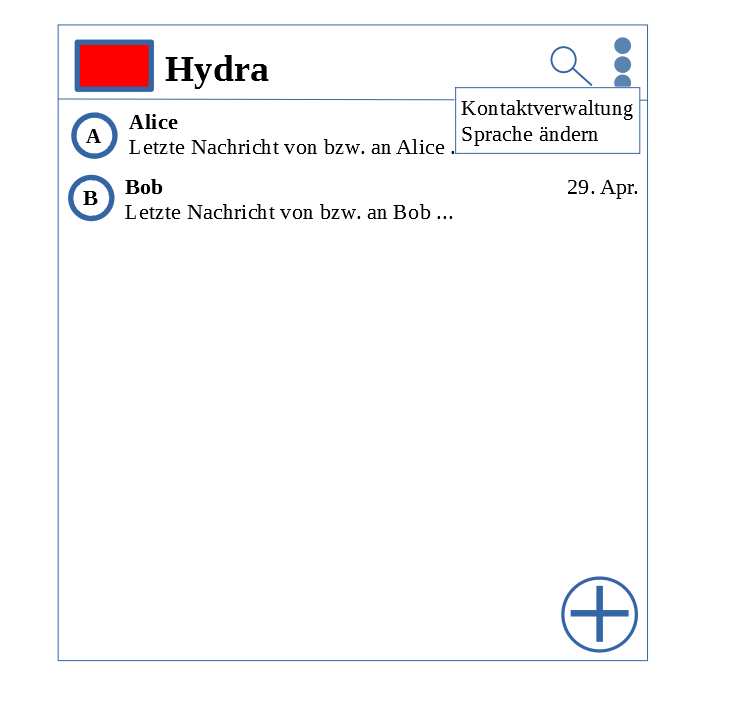
\includegraphics[scale=0.3]{gui/Startseite_mit_Einstellungen.png}
  \caption{Startseite mit Einstellungen}
\end{subfigure}
\caption{GUI Startseite}
\end{figure}

Startseite:\\
Die Lupe oben links ermöglicht die Volltextsuche.\\
Die drei vertikal angeordneten Punkte öffnen die Einstellungen.\\
Anwählen von z.B. Alice öffnet den Chat mit Alice.\\
Das Plus-Symbol unten rechts öffnet die Kontaktverwaltung.\\
\newpage

\begin{figure}[h]
\centering
\begin{subfigure}{.5\textwidth}
  \centering
  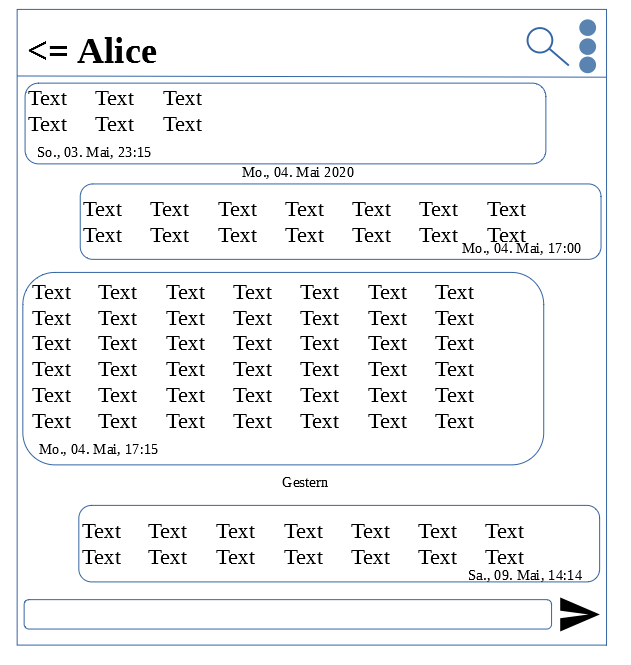
\includegraphics[scale=0.3]{gui/Chatfenster.png}
  \caption{Chatfenster}
\end{subfigure}%
\begin{subfigure}{.5\textwidth}
  \centering
  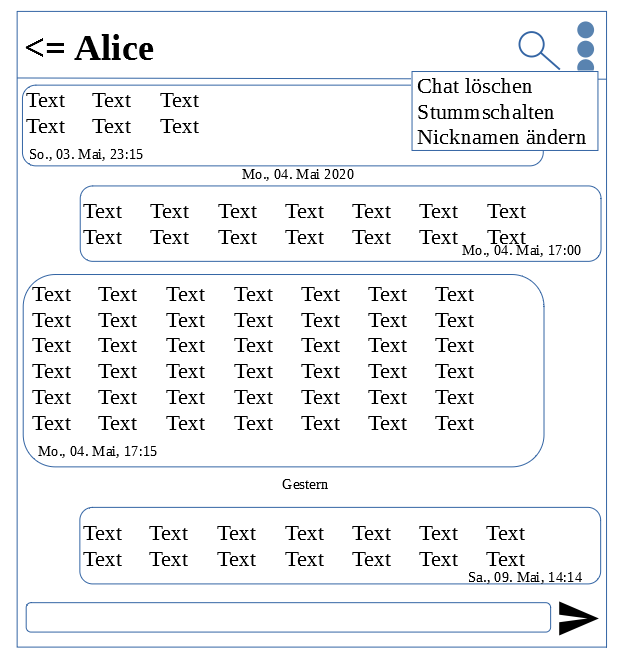
\includegraphics[scale=0.3]{gui/Chatfenster_mit_Einstellungen.png}
  \caption{Chatfenster mit Einstellungen}
\end{subfigure}
\caption{GUI Chatfenster}
\end{figure}

Chatfenster:\\
Die Lupe oben links ermöglicht die Volltextsuche in diesem Chat.\\
Im Chatfenster öffnen die drei vertikal angeordneten Punkte die Chat-Einstellungen.\\
Anwählen der Leiste am unteren Bildschirmrands ermöglicht die Eingabe einer Nachricht.\\
Der Pfeil am unteren rechten Rand versendet die Verfasste Nachricht.\\

\newpage

\begin{figure}[h]
\centering
\begin{subfigure}{.5\textwidth}
  \centering
  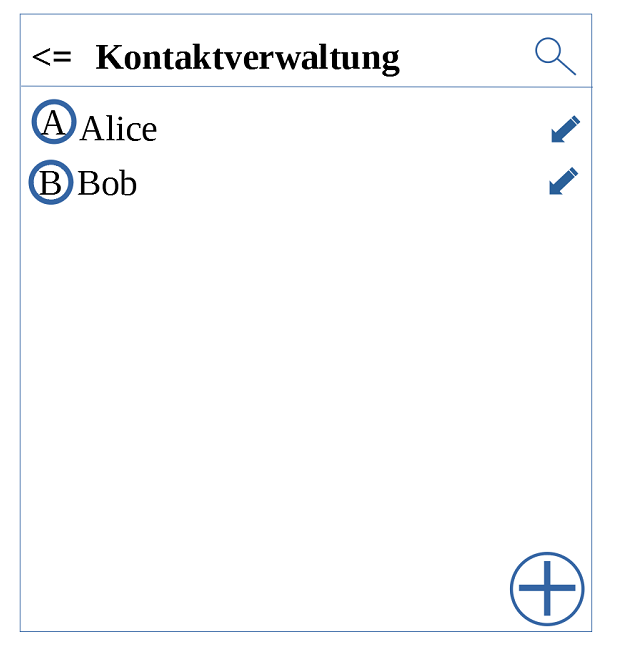
\includegraphics[scale=0.3]{gui/Kontaktverwaltung.png}
  \caption{Kontaktverwaltung}
\end{subfigure}%
\begin{subfigure}{.5\textwidth}
  \centering
  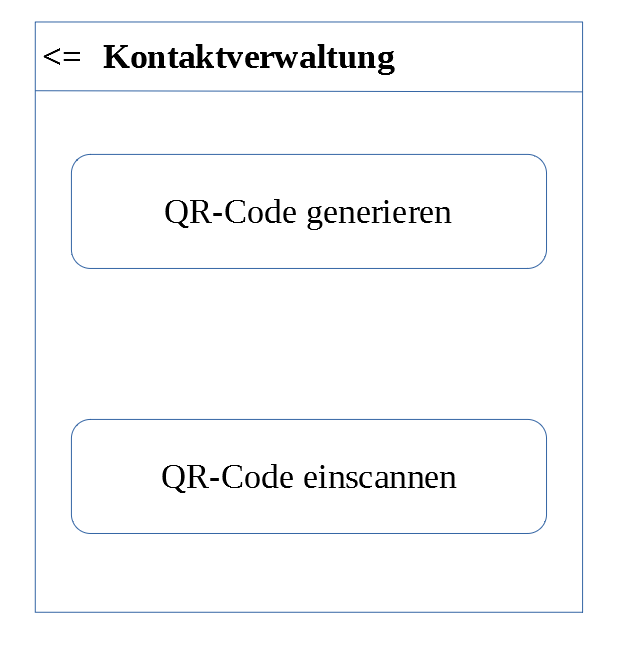
\includegraphics[scale=0.3]{gui/Kontaktverwaltung_QR_Code.png}
  \caption{Kontaktverwaltung QR-Code}
\end{subfigure}
\caption{GUI Kontaktverwaltung}
\end{figure}

Kontaktverwaltung:\\
In der Kontaktverwaltung kann man durch anwählen eines Kontaktes den zugehörigen Chat öffnen bzw. falls noch keiner existiert diesen starten.\\
Der Stift am rechten Rand lässt den Benutzer das Pseudonym des Kontaktes ändern.\\
Das Plus-Symbol unten rechts ermöglicht es dem Benutzer neue Kontakte hinzuzufügen.\\

\begin{figure}[h]
\centering
\begin{subfigure}{.5\textwidth}
  \centering
  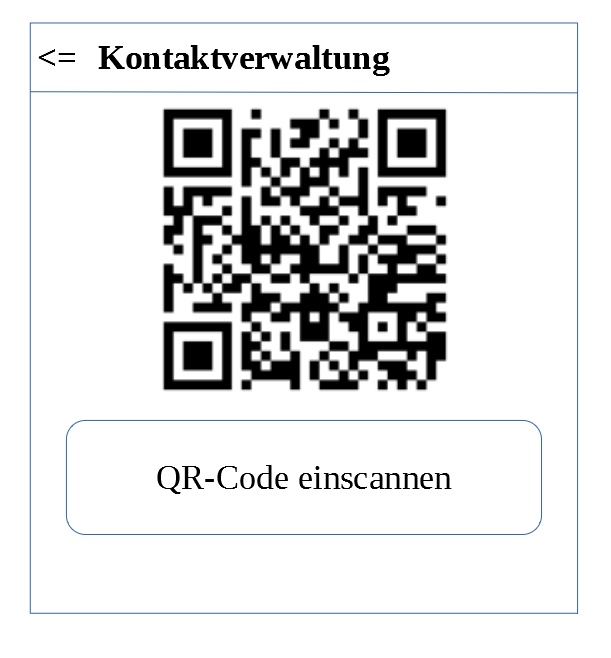
\includegraphics[scale=0.3]{gui/Kontaktverwaltung_QR_Code_generiert.png}
  \caption{Generierter QR-Code}
\end{subfigure}%
\begin{subfigure}{.5\textwidth}
  \centering
  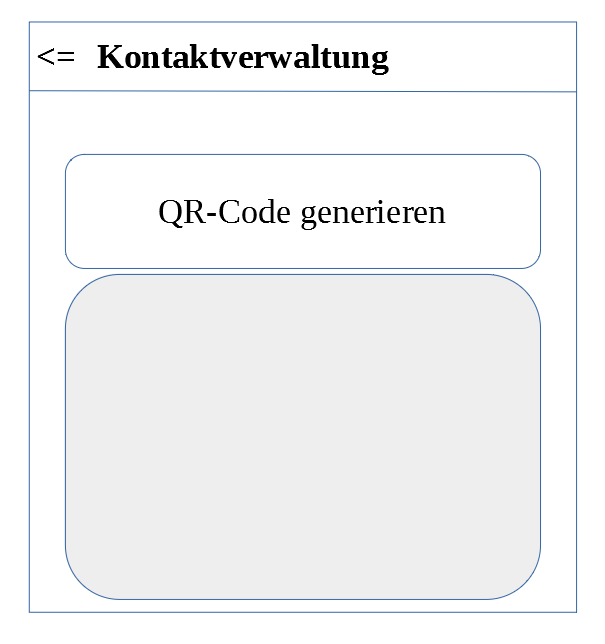
\includegraphics[scale=0.3]{gui/Kontaktverwaltung_QR_Code_einscannen.png}
  \caption{QR-Code einscannen}
\end{subfigure}
\caption{GUI QR-Code}
\end{figure}


\newpage




 \newpage
  \section{Abkürzungsverzeichnis}

\begin{acronym}
\acro{DS}[DS]{Directory Service}

\acro{HC}[HC]{Hydra-Client}
\acro{HS}[HS]{Hydra-System}
\acro{GUI}[GUI]{Grafische Benutzeroberfläche}

\acro{gRPC}[gRPC]{Remote Procedure Calls}
\acro{OE}[OE]{onion-encryption}
\acro{ECDH}[x448-ECDH]{x448 Elliptic-curve Diffie–Hellman}
\acro{AES}[AES]{AES 256B Galois/Counter Mode}
\acro{CS}[CS]{Contact Service}
\acro{CC}[CC]{Circuit Cell}

\acro{E2EE}[E2EE]{Ende-zu-Ende Verschlüsselung}
\acro{MS}[MS]{Main-Service}
\acro{NDK}[NDK]{Android Native Development Kit}
\acro{JNI}[JNI]{Java Native Interface}

\acro{MVC}[MVC]{Model-View-Controller}
\acro{HCB}[HCB]{Hydra Core Bibliothek}

\acro{CSQ}[CSQ]{Cell-Send-Queue}
\acro{CRQ}[CRQ]{Cell-Receive-Queue}

\acro{DP}[DC]{Dummy Cell}

\end{acronym} \newpage
\end{document}
